\section{ORS-Experiment mit einer Weißlichtquelle}\label{sec:versuchsteil2}
\subsection{Aufbau}\label{subsec:teil2_aufbau}
In diesem Versuchsteil wird die OPP-Dispersionsrelation anhand einer Silber-Luft-Grenzfläche vermessen. Dazu wird eine Weißlichtquelle (Licht
bestehend aus mehreren Wellenlängen) und ein Spektrometer verwendet. Der Versuchsaufbau dieses Versuchsteils ähnelt dem des ersten Versuchsteils und ist
in \cref{fig:versuchsteil2_aufbau} dargestellt. Die Funktion einzelner Bauteile wird nun nicht erneut erklärt (für kurze Erklärungen siehe \cref{subsec:teil1_aufbau}).
\begin{figure}[H]
	\centering
	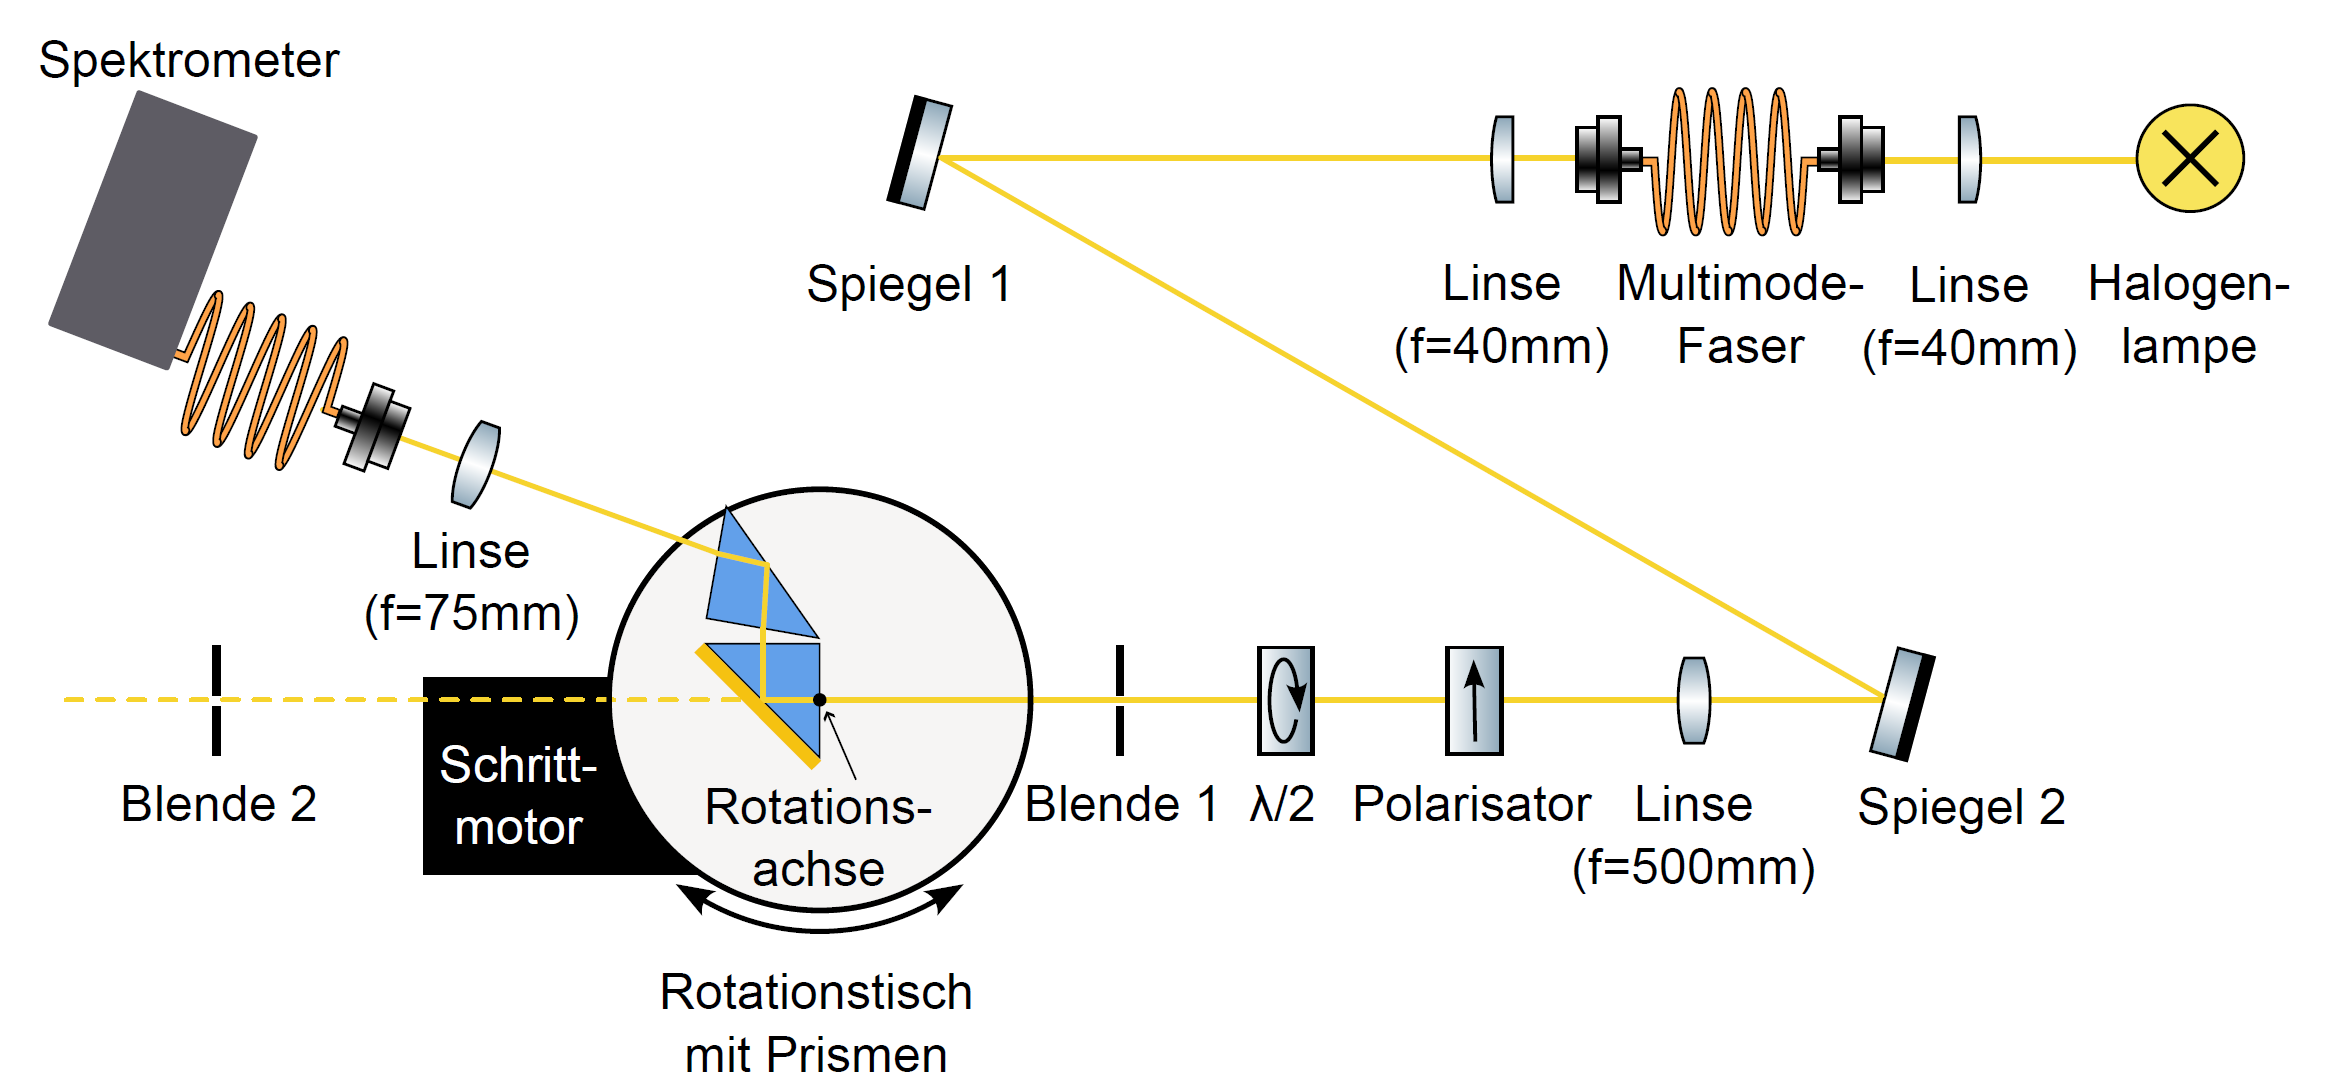
\includegraphics[width=0.6\linewidth]{../figs/versuchsteil2_aufbau.png}
	\caption{Versuchsaufbau des ORS-Experiments mit einer Weißlichtquelle und einer Zwei-Prismen-\\Konfiguration (hier ist die Linse vor der
    Multimode-Faser vor dem Spektrometer durch ein Objektiv zu ersetzen) \cite{skript}.}
	\label{fig:versuchsteil2_aufbau}
\end{figure} Als Weißlichtquelle wird eine Halogenlampe verwendet. Diese ist bereits auf dem optischen Tisch montiert. Zuerst wird das Licht der
Lampe mithilfe einer Sammellinse der Brennweite $f = \SI{40}{\mm}$ in eine Multimode-Faser gekoppelt. Diese Multimode-Faser wird verwendet, um eine
möglichst homogene Ausleuchtung zu erreichen. Vor dem Laser des ersten Versuchsteils wird dann die Ausgangsseite der Multimode-Faser platziert, wobei
die Höhe des Faserauskopplers auf etwas \SI{10}{\cm} eingestellt wird. Anschließend wird eine Sammellinse mit der Brennweite $f = \SI{40}{\mm}$ vor
den Faserauskoppler gestellt, um den Lichtstrahl zu kollimieren. Dieser Lichtstrahl muss nun analog zu dem ersten Versuchsteil justiert werden. Dafür
wird der Rotationstisch entfernt. Wieder werden die beiden Spiegel verwendet, den Lichtstrahl iterativ durch die beiden Blenden zu justieren. Hierfür
werden vorerst die Wellenplatte, der Polarisator und die Linse aus dem Strahlengang genommen und nach der Justierung des Lichtstrahls durch die beiden
Blenden wieder an die entsprechenden Positionen eingesetzt. Hierbei muss darauf geachtet werden, dass der Lichtstrahl nach dem Einsetzen der Wellenplatte,
des Polarisators und der Linse weiterhin durch beide Blenden verläuft. Nun wird auch wieder der Rotationstisch auf die vorgesehene Stelle auf dem optischen
Tisch platziert. Die Photodiode wird nun durch ein Spektrometer ersetzt, um das reflektierte Spektrum der Weißlichtquelle messen zu können.
Das reflektierte Licht wird über eine Multimode-Faser in das Spektrometer gekoppelt. Außerdem wird die Linse, die bei dem ersten Versuchsteil vor der Photodiode stand,
durch ein Objektiv ersetzt. Um die Einkopplung des Lichtstrahls in die Multimode-Faser zu optimieren, wird das Programm \texttt{ORSScan} benutzt. Da
das Spektrometer sättigt, wird die Intensität mit der Blende 1 angepasst.
\subsection{Messung}\label{subsec:teil2_messung}
Bereits vor dem Aufbau dieses Versuchsteils wurde gemeinsam mit dem Assistenten
\subsection{Auswertung}\label{subsec:teil2_auswertung}